\subsection{Player ratings}

The player ratings provided by \whoscored\ are calculated using over 200 statistics, and provide an accurate measure on a player's contributions to the team \\ \citep{bib:whoscored-ratings}. The player ratings are adjusted throughout the whole match. Every event of importance is taken into account when calculating the rating.

Before using player ratings for predicting match outcome, one should confirm that the ratings actually have predictive properties. To confirm this, a simple \gls{fnn} with one hidden layer of 64 nodes, activated using \gls{relu} was set up. The network takes in the final rating of the 22 starting players for each match. \cref{fig:network-player-ratings-to-result} shows the network structure. 

The input values $I_{1}, ..., I_{22}$ are the final ratings for the 22 starting players, divided by $10$ to map them to the range $[0, 10]$. The players are first ordered by team. The first 11 input values are players from the home team, and the next 11 are from the away team. The players in each team are also ordered, first by $x$ position on the field, then by $y$ position on the field. The position $(0, 0)$ is at each team's right corner flag. This makes the keeper the first player, and the forwards the last.

For the match between Arsenal and Manchester United May 7, 2017, shown in \cref{fig:arsenal-manchester-united-player-ratings}, the input values would be as follows:
\begin{lstlisting}[language=Python]
    [0.76, 0.70, 0.74, 0.68, 0.81, 0.72, 0.75, 0.73, 0.72, 0.70, 0.77, 0.60, 0.67, 0.62, 0.65, 0.66, 0.65, 0.67, 0.61, 0.69, 0.66, 0.65]
\end{lstlisting}

\begin{figure}
    \centering
    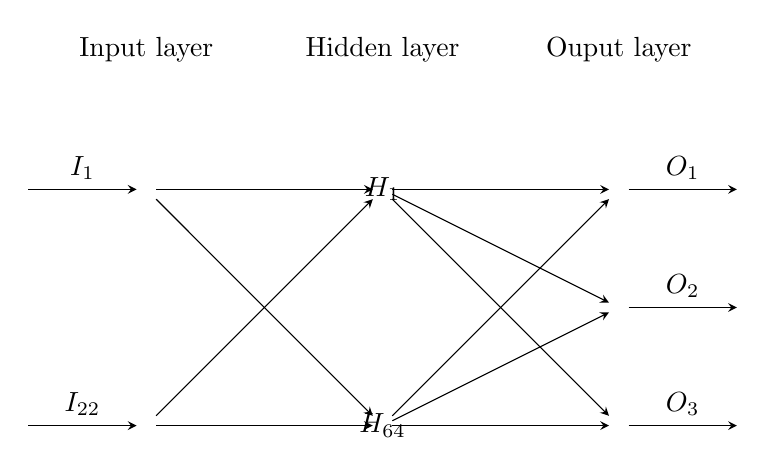
\begin{tikzpicture}[x=1.5cm, y=1.5cm, >=stealth]
        %%%%%%%%%%%%%%%%%%%%%%%%%%%%%%%%%%%%%%%%%%%%
        % Input nodes
        %%%%%%%%%%%%%%%%%%%%%%%%%%%%%%%%%%%%%%%%%%%%
        
        % Drawing
        \foreach \m/\l [count=\y] in {1,missing,2}
            \node [every neuron/.try, neuron \m/.try] (input-\m) at (0,2-\y) {};

        % Labeling
        \foreach \l [count=\i] in {1,22}
            \draw [<-] (input-\i) -- ++(-1,0)
                node [above, midway] {$I_{\l}$};
        
        
        %%%%%%%%%%%%%%%%%%%%%%%%%%%%%%%%%%%%%%%%%%%%
        % Hidden nodes
        %%%%%%%%%%%%%%%%%%%%%%%%%%%%%%%%%%%%%%%%%%%%
        
        % Drawing
        \foreach \m [count=\y] in {1,missing,2}
            \node [every neuron/.try, neuron \m/.try ] (hidden-\m) at (2,2-\y) {};
        
        % Labeling
        \foreach \l [count=\i] in {1,64}
            \node at (hidden-\i) {$H_{\l}$};
        
        
        %%%%%%%%%%%%%%%%%%%%%%%%%%%%%%%%%%%%%%%%%%%%
        % Output nodes
        %%%%%%%%%%%%%%%%%%%%%%%%%%%%%%%%%%%%%%%%%%%%
        
        % Drawing
        \foreach \m [count=\y] in {1,...,3}
            \node [every neuron/.try, neuron \m/.try ] (output-\m) at (4,2-\y) {};
        
        % Labeling
        \foreach \l [count=\i] in {1,...,3}
            \draw [->] (output-\i) -- ++(1,0)
                node [above, midway] {$O_{\l}$};
        
        
        %%%%%%%%%%%%%%%%%%%%%%%%%%%%%%%%%%%%%%%%%%%%
        % Connecting
        %%%%%%%%%%%%%%%%%%%%%%%%%%%%%%%%%%%%%%%%%%%%
        
        % Input nodes to hidden nodes
        \foreach \i in {1,...,2}
            \foreach \j in {1,...,2}
                \draw [->] (input-\i) -- (hidden-\j);
        
        % Hidden nodes to output nodes
        \foreach \i in {1,...,2}
            \foreach \j in {1,...,3}
                \draw [->] (hidden-\i) -- (output-\j);
        
        
        %%%%%%%%%%%%%%%%%%%%%%%%%%%%%%%%%%%%%%%%%%%%
        % Labeling layers
        %%%%%%%%%%%%%%%%%%%%%%%%%%%%%%%%%%%%%%%%%%%%
        \foreach \l [count=\x from 0] in {Input, Hidden, Ouput}
            \node [align=center, above] at (\x*2,2) {\l\ layer};
    \end{tikzpicture}
    \caption{Player ratings network structure.}
    \label{fig:network-player-ratings-to-result}
\end{figure}

\begin{figure}
    \centering
    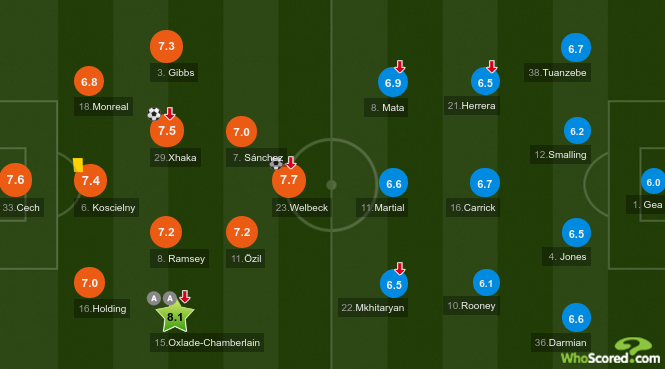
\includegraphics[width=\textwidth]{experimental-setup/arsenal-manchester-united-player-ratings.png}
    \caption{The final ratings for the players starting the match between Arsenal and Manchester United May 7, 2017.}
    \label{fig:arsenal-manchester-united-player-ratings}
\end{figure}

The network can with $90\%$ certainty predict the match outcome (averaged over ten network instances), yielding an average \gls{rps} of $0.0394$. This indicates the player ratings say a lot about the final rating.

\subsubsection{Input}

As the final ratings are not known at match start, ratings from previous matches must be used. For each starting player, the three most recent matches are taken into consideration. The following values from the three previous matches of each player are added to the model input:
\begin{itemize}[noitemsep]
    \item Player's final rating.
    \item Portion of the match played: The number of minutes played divided by $120$. This is added in order to increase the impact of players playing the whole match. 120 is used instead of 90 to support matches that might go to extra time.
    \item Player's team's final rating. This is added to capture cases where the player rating are affected by of the team's collective effort.
    \item Other team's final rating. This is added to capture cases where the player rating are affected by of the other team's collective effort.
    \item A Boolean value, indicating whether the player played at home or away. This is added to take the home ground advantage into consideration.
    \item Days since the match, $exp(-\text{days since match} / 7)$. This is added in order to increase the impact of more recent matches.
\end{itemize}

In addition to the previous match features, the number of matches the last two game weeks are added for each player. That gives $3 * 6 + 1 = 19$ features for each player. With $22$ players, there are $22 * 19 = 418$ features per match.